
\chapter{Introduction}\label{C:intro}

According to Bertino \cite{Bertino2012} \emph{Version control systems} provide a way of allowing multiple developers to collaborate. When multiple developers work on the same source code there is a risk that they have conflicting changes for the same portion of the source code.  One way of managing these conflicting changes is by ensuring only one person can edit a file at a time. This locking mechanism was recommended by Tichy \cite{Tichy1982} for the RCS version control system. Of course, the problem here is that one person can stop others from being able to edit the file. 

An alternative approach is to allow multiple changes to a file and to automatically resolve most of them in a process called a \emph{merge}.  The merge process compares the changes made in one version with the changes made on the other version. If the merge process determines that changes can coexist, it creates a merged file that contains all the changes. The changes that cannot be automatically merged are known as \emph{merge conflicts}.  The merge conflicts need to be manually checked and edited to form a merged file with the correct changes.

\begin{figure}[!t]
 \begin{center}
 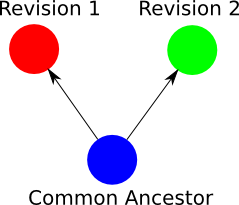
\includegraphics[scale=1]{introRevisions}
 \end{center}
 \caption{A file that has two different revisions}
 \label{fig:introRevisions}
\end{figure}



Internally the merge process needs to determine what changes have happened to both of the revisions being compared. In Figure  ~\ref{fig:introRevisions} there are two revisions that are derived from a common ancestor. It is possible to determine what has been deleted, inserted or changed by comparing each of the revisions against the common ancestor.  This is often done as a linear comparison of the source code for each revision. This works very well provided there has been no change in the order or structure of the file. However, if there has been a change where a block of source code has been moved from one place to another a linear comparison instead determines that two changes have occurred.  This is equivalent to deleting a block of source code from the common ancestor and inserting that source code elsewhere. It is possible that this change is not important to other programmers as the program behaves in the same manner even when source code is in a different order.  An example of this is if a Java programmer changes the order of methods within a program.  The program will behave in the same way as changing the order of methods does not change any functionality, however the source code is now different. The swapping of the order of the method is still counted as being two different changes even though the program behaves in the same manner as it did before the change took place.

Without any further analysis this change is recorded in the merged file even if the reordering was a personal preference for the programmer.  Although there has been no functional change the version control system will treat the relocation of blocks of source code exactly like a change in functionality.  Whenever a programmer attempts to update their code to incorporate any change in functionality, the change to the order of methods is also made to their code.  If a programmer is already familiar with the old structure of code and expects the code to remain relatively consistent the swapping of methods could be disconcerting.

Another issue that non-functional changes raise is an increase in the number of \emph{merge conflicts}. This could occur when two views have had a small amount of refactoring.  Since in both views the behaviour of the program has not changed it is possible that the merge conflict occurs about something trivial. An example of this could be different formatting or ordering methods alphabetically. For an ordinary text merge these changes to the structure of the source code require manual intervention. These issues highlight the need to develop smarter ways to merge.

It is becoming more important to have smarter merges because of the scale of many software projects and the number of developers working on them.
Large online repositories, like GitHub, contain many open source projects.
It is possible for these projects to make source code available to many developers at a time.
This means it is possible for two developers to work on the same project while having little personal contact.
Care needs to be taken when their individual work is combined.
Preferably most of the problems with merging their work should be automatically resolved however,
there still could be instances where either or both developers will have to figure out how the code should interact.
Having better automatic merges reduces the risk that time will be spent manually figuring out how different changes should be combined.

This thesis introduces the concept of maintaining multiple separate views which can be ordered differently but have functionally equivalent source code.
The purpose of these views is to reduce the number of changes introduced during a merge. 
It also explores a way of allowing a version control system to detect when there is a change in the source code but not a functional change in a program.
Examples of this are if items have been reordered, if comments have been inserted or there have been changes to the formatting. 
We developed the Refactor Categories Tool for the purpose of identifying these changes. 
We report on the design and implementation of this tool.
The Refactor Categories Tool is then used in an experiment evaluating a range of real-world benchmarks.


% We have used the Refactor Categories Tool we have created in an expiriment 
% that iterates though all the revisions in the versi on source control for a 
% handful of Java projects.
% The Refactor Categories Tool detects
% 
% need to write about what we found here
 

\section{Overview}
In this thesis we explore the idea of having private views that although functionally equivalent can be refactored differently.
A version control system allows us to have 
In this thesis we will examine the effects of non functional changes caused by light weight refactoring of code on version control systems.
To do this we will examine version control systems and how they allow collaboration through merging.
We will also examine refactoring and how it can change the code but retain the same behaviour.
We will some tools that could help when merging refactored code when it is checked into an operating system. 
We especially focus on JDime to see if I can help us to build a private view where external code changes are minimised.
 
